% These are the lecture notes for my CSCI360 course SPRING 2017
% at John Jay College of Criminal Justice. They are based largely on
% Schneier's Applied Cryptography.

% Feel free to edit these slides and use them for your own courses.
% HOWEVER DO NOT REMOVE THESE LINES!
% Email me at: awood [at] jjay.cuny.edu
% or at: awood [at] gradcenter.cuny.edu


\documentclass{beamer}

\usepackage{tikz}
\usetikzlibrary{calc}

\usepackage{forest}
\usepackage{verbatim}
\usepackage{color}
\usepackage{amsmath}
\usepackage{graphicx}
\usepackage{caption}



\setbeamertemplate{footline}[frame number]
\setbeamertemplate{navigation symbols}{} 

\newtheorem{thm}{Theorem}[section]
\newtheorem{lem}{Lemma}
\newtheorem{cl}{Claim}
\newtheorem{cor}{Corollary}[section]
\newtheorem{conj}{Conjecture}
\newtheorem{quest}{Question}
\newtheorem{defn}{Definition}[section]
\newtheorem{obs}{Observation}[section]
\newtheorem{exam}{Example}

\newcommand{\im}{\operatorname{im}}
\newcommand{\id}{\operatorname{id}}
\newcommand{\interior}{\operatorname{int}}
\newcommand{\bdry}{\operatorname{bdry}}
\newcommand{\<}{\langle}
\renewcommand{\>}{\rangle}
\newcommand{\Gab}{(G_\phi)^{ab}} 
\newcommand{\phibar}{\bar{\phi}}
\newcommand{\Z}{\mathbb{Z}}
\newcommand{\N}{\mathbb{N}}
\newcommand{\Q}{\mathbb{Q}}
\newcommand{\R}{\mathbb{R}}
\newcommand{\C}{\mathbb{C}}
\newcommand{\A}{\mathcal{A}}
\newcommand{\OO}{\mathcal{O}}
\newcommand{\UU}{\mathcal{U}}
\newcommand{\power}{2^{\{P_1, \cdots , P_n\}}}
\newcommand{\bp}{\begin{problem}}
\newcommand{\ep}{\end{problem}}
\newcommand{\ba}{\begin{answer}}
\newcommand{\ea}{\end{answer}}
\newcommand{\ds}{\displaystyle}
\newcommand{\ben}{\renewcommand{\theenumi}{\alph{enumi}}
\renewcommand{\labelenumi}{(\theenumi)}\begin{enumerate}}
\newcommand{\een}{\end{enumerate}}
\newcommand{\Hess}{\operatorname{Hessian}}
\newcommand{\Aut}{\mathrm{Aut}}
\newcommand{\Inn}{\mathrm{Inn}}
\newcommand{\Out}{\mathrm{Out}}
\newcommand{\End}{\mathrm{End}}


\mode<presentation>
{
%  \usetheme{default}
  \setbeamercovered{invisible}
}


\usepackage[english]{babel}
\usepackage[latin1]{inputenc}
\usepackage{times}
\usepackage[T1]{fontenc}
\usepackage{stmaryrd}

%\usetheme{default}
%\usetheme{AnnArbor}
%\usetheme{Antibes}
%\usetheme{Bergen}
%\usetheme{Berkeley}
%\usetheme{Berlin}
%\usetheme{Boadilla}
%\usetheme{CambridgeUS}
%\usetheme{Copenhagen}
%\usetheme{Darmstadt}
%\usetheme{Dresden}
%\usetheme{Frankfurt}
%\usetheme{Goettingen}
%\usetheme{Hannover}
%\usetheme{Ilmenau}
%\usetheme{JuanLesPins}
%\usetheme{Luebeck}
%\usetheme{Madrid}
%\usetheme{Malmoe}
%\usetheme{Marburg}
%\usetheme{Montpellier}
%\usetheme{PaloAlto}
%\usetheme{Pittsburgh}
%\usetheme{Rochester}
\usetheme{Singapore}
%\usetheme{Szeged}
%\usetheme{Warsaw}

%\usecolortheme{default}
%\usecolortheme{albatross}
\usecolortheme{beaver}
%\usecolortheme{beetle}
%\usecolortheme{crane}
%\usecolortheme{dolphin}
%\usecolortheme{dove} % grey, white, yellow
%\usecolortheme{fly} %grey, yellow
%\usecolortheme{lily} %white, yellow, blue
%\usecolortheme{orchid}
%\usecolortheme{rose}
%\usecolortheme{seagull}
%\usecolortheme{seahorse}
%\usecolortheme{whale}
%\usecolortheme{wolverine}

% Title page

\title[LEA]{Length Extension Attacks}

\author
{Lecture notes of Alexander Wood \\ \scriptsize \href{mailto:awood@jjay.cuny.edu}{awood@jjay.cuny.edu}}
\institute[JJay]{John Jay College of Criminal Justice}  

\date{}

\begin{document}

% Remove 'figure' text from figure captions 
\setbeamertemplate{caption}{\raggedright\insertcaption\par}

\begin{frame}
  \titlepage
\end{frame}


\begin{frame}
\frametitle{MACs: Review}

A \textbf{message authentication code (MAC)} is a key-dependent one-way hash function.
\newline

They satisfy the same properties as one-way hash functions. In addition they have a \textbf{key}.\newline

MACs are used to \textbf{authenticate} files between users. It checks its \textbf{authenticity} (confirms the sender) as well as its \textbf{integrity} (it has not been tampered with). \newline
\end{frame}


\begin{frame}
\frametitle{MAC Visualization}

\begin{figure}
\centering
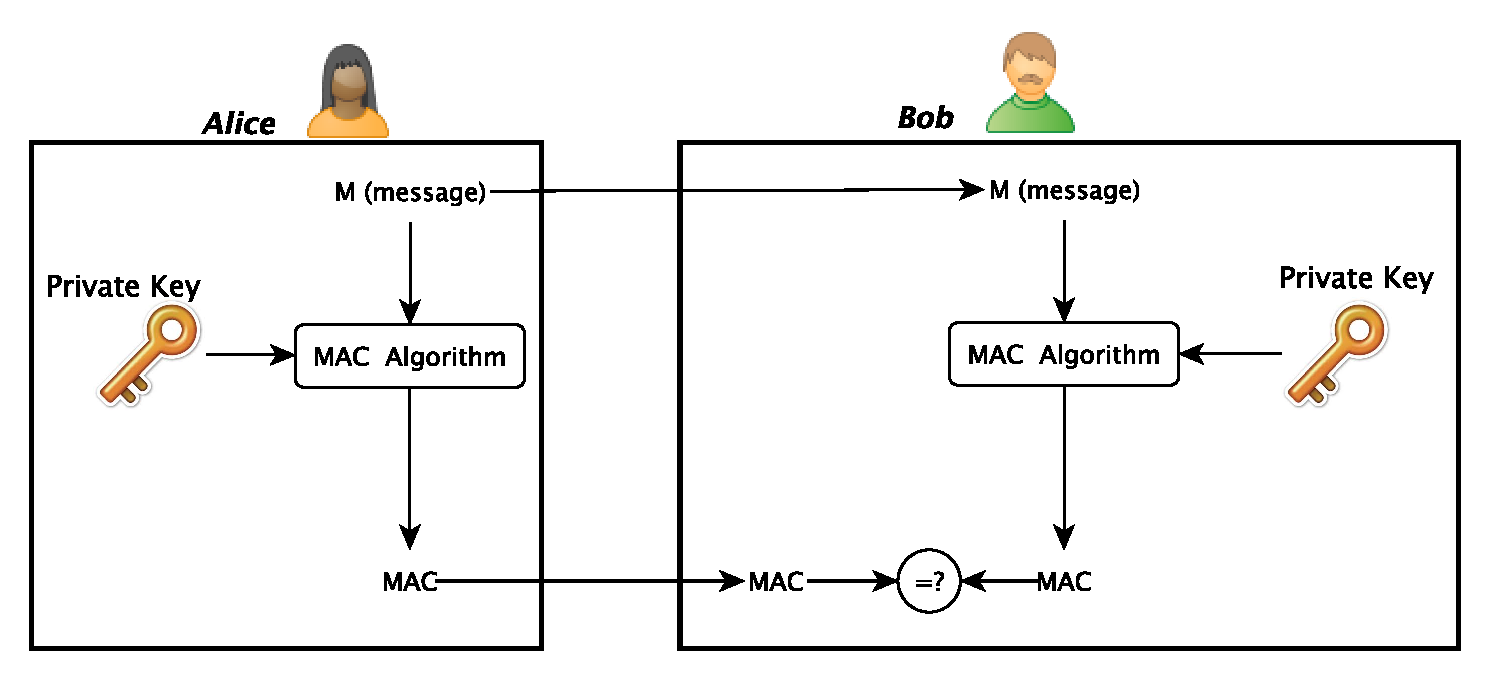
\includegraphics[scale=.45]{IMG/MAC}
\end{figure}
\end{frame}

\begin{frame}[fragile]
\frametitle{MAC Algorithms}

\begin{itemize}
\item \verb|KeyGen| - generates a key $1^n$ uniformly at random.
\item \verb|Sign| - Alice inputs her key $k$ and message $M$, receives output $t$ (tag).
\item \verb|Verify| - Bob verifies the authenticity of Alice's message.
\end{itemize}
\end{frame}


\begin{frame}
\frametitle{Merkle-Damgard Construction}

We should now be familiar with the \textbf{Merkle-Damgard Construction} of a hash function.

\begin{figure}
\centering
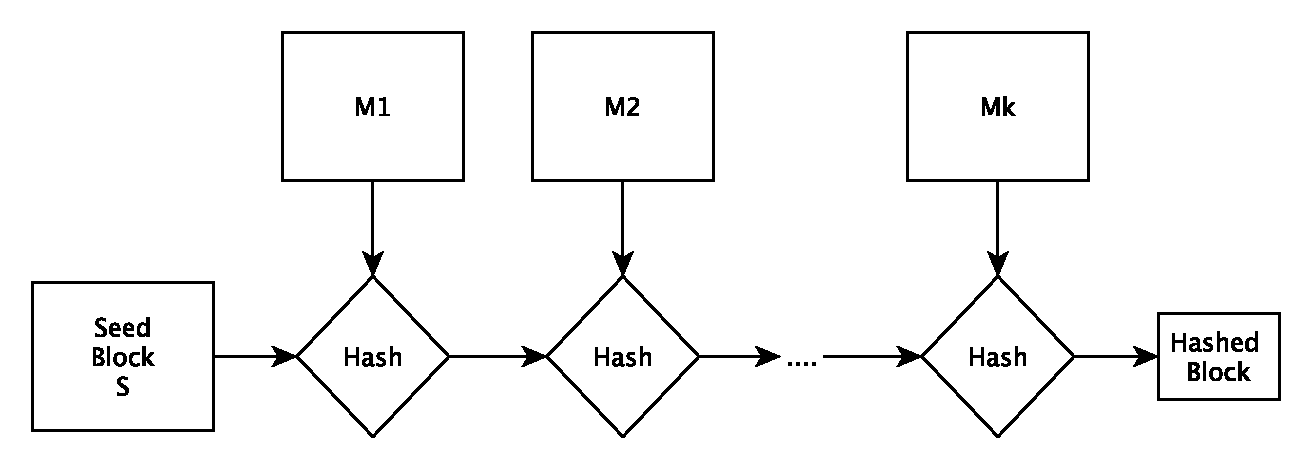
\includegraphics[scale=.5]{IMG/hash3}
\end{figure}
\end{frame}


\begin{frame}
\frametitle{CBC-MAC}

MACs can be constructed similarly by including a \textbf{key}. Recall that this is called \textbf{CBC-MAC}.

\begin{figure}
\centering
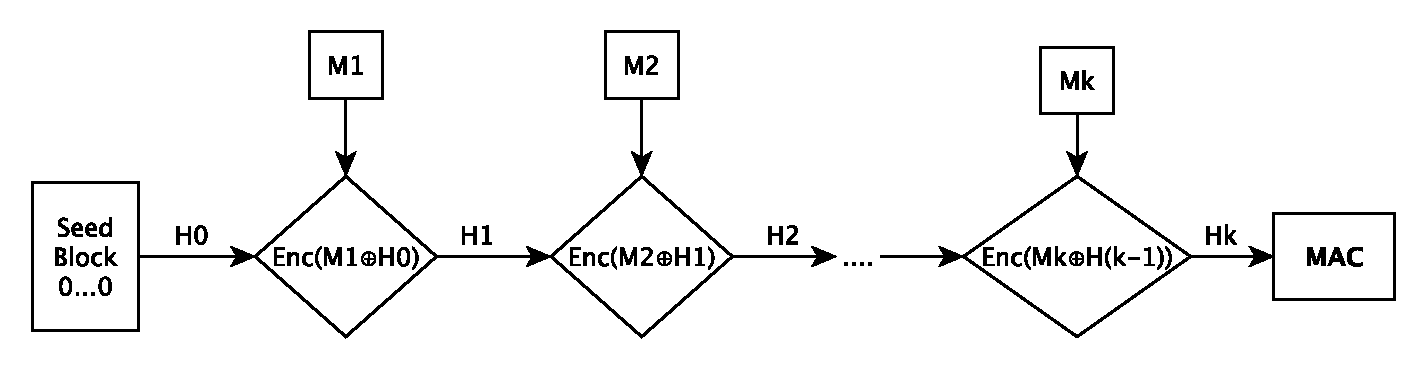
\includegraphics[scale=.45]{IMG/CBCMACchain}
\end{figure}
\end{frame}


\begin{frame}
\frametitle{CBC-MAC}

CBC-MAC is secure for fixed-length messages \emph{if the underlying block cipher used is secure}.
\end{frame}


\begin{frame}
\frametitle{Length-Extension Attacks}

Today we look at a different attack, the \textbf{length extension attack}. This attack works specifically against \textbf{Merkle-Damgard based hashes} which are inappropriately used as MACs.\newline

Thus, algorithms like MD5, SHA-1, and SHA-2 are susceptible. SHA-3 and HMAC are not susceptible to this form of attack. 
\end{frame}


\begin{frame}
\frametitle{Length-Extension Attacks}

A length extension attack is carried out as follows. Let $H$ be a hash function and $M_1$ a message.
\begin{itemize}
\item An attacker, Eve, intercepts $H(M_1)$, the hash of message 1. Let $L$ be the length of $M_1$. 
\item Eve calculates $H(M_1 \| M_2)$ for a message $M_2$ of her choosing.
\item The value $H(M_1\| M_2)$ now verifies as signed by the original sender.
\end{itemize}
\end{frame}

\begin{frame}
\frametitle{SHA-1: Length Extension Attack}

Recall that SHA-1 uses 512-bit blocks. In order to send a message, it is first \textbf{padded} in order to be a multiple of 512 bits. 

\begin{figure}
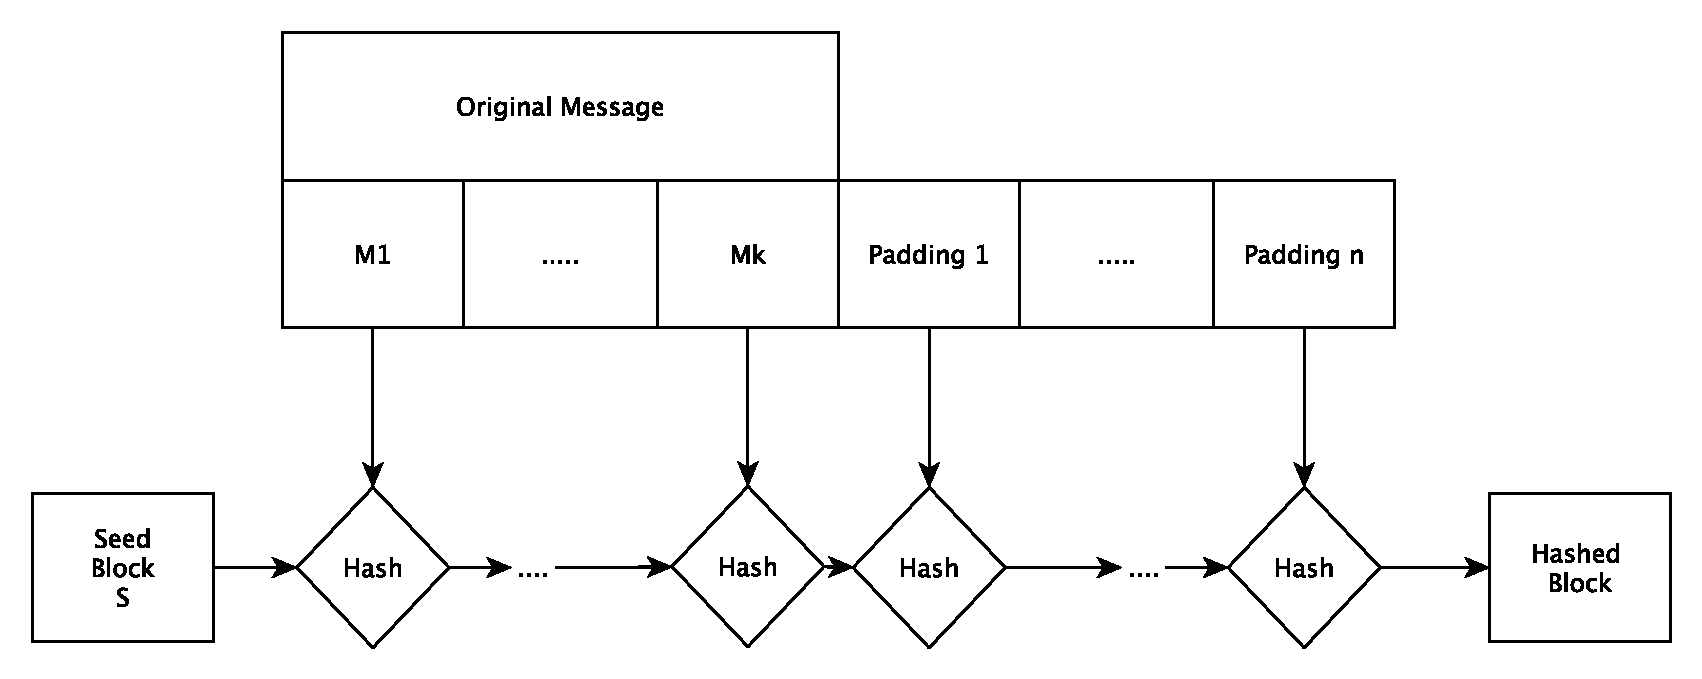
\includegraphics[scale=.4]{IMG/padding}
\end{figure}
\end{frame}

\begin{frame}
\frametitle{SHA-1: Length Extension Attack}

Eve intercepts the hashed block, $H$. She knows:
\begin{itemize}
\item The hashed block $H$, which is the hash on the message $M_1 \| P$ for some padding $P$.
\item The message $M_1 \| P$.
\item The length of the key $K$.
\end{itemize}
\end{frame}


\begin{frame}
\frametitle{SHA-1: Length Extension Attack}

Let $M' = M_1 \| P \| M_2$. Pad this further to make it a multiple of $512$ bits. Eve can now compute the hash of $M'\| H'$.
\begin{figure}
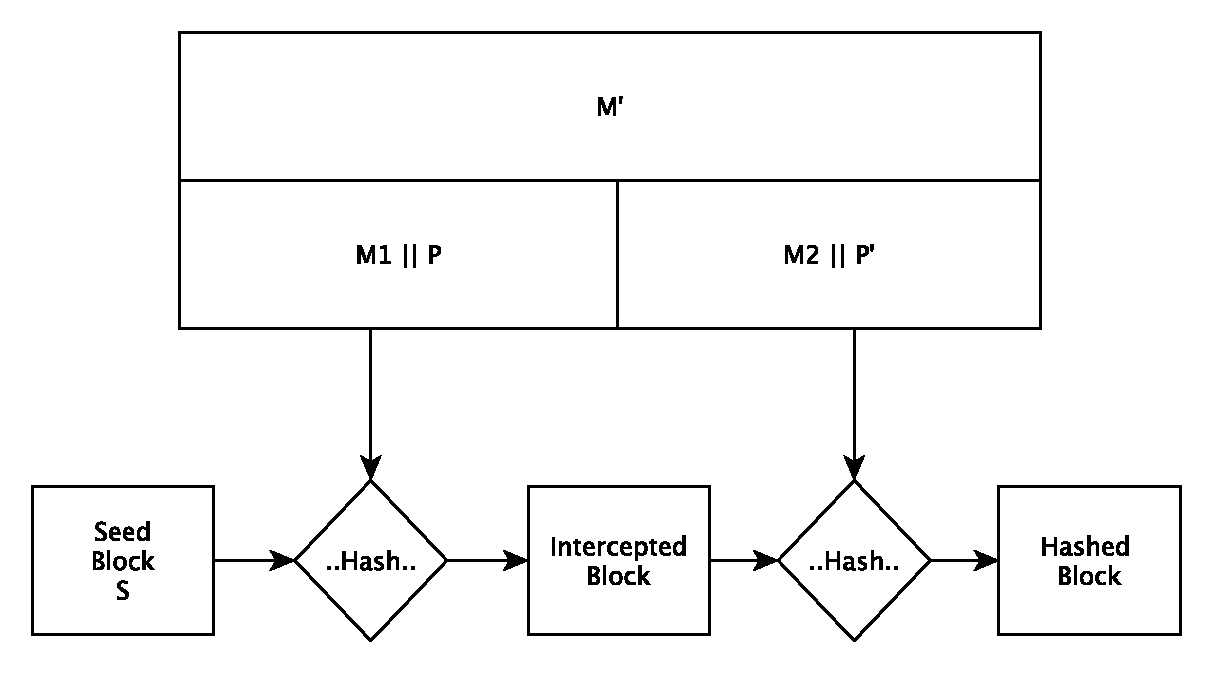
\includegraphics[scale=.5]{IMG/lenghtextattack}
\end{figure}
\end{frame}

\begin{frame}[fragile]
\frametitle{SHA-1: Length Extension Attack}

How can Eve use this to her advantage? Suppose a MAC is built using SHA-1.
\begin{itemize}
\item \verb|Sign|: Alice signs a message $M$ with a key $K$ by computing the value $S=$ \verb|SHA1|$(K\| M)$.
\item \verb|Verify|: Bob verifies the message $M$ by computing \verb|SHA1|$(K \|M)$ and verifying that this is is equal to the signature $S$ sent by Alice.
\end{itemize}
\end{frame}

\begin{frame}
\frametitle{SHA-1: Length Extension Attack}

This MAC protocol would work as follows.
\begin{figure}
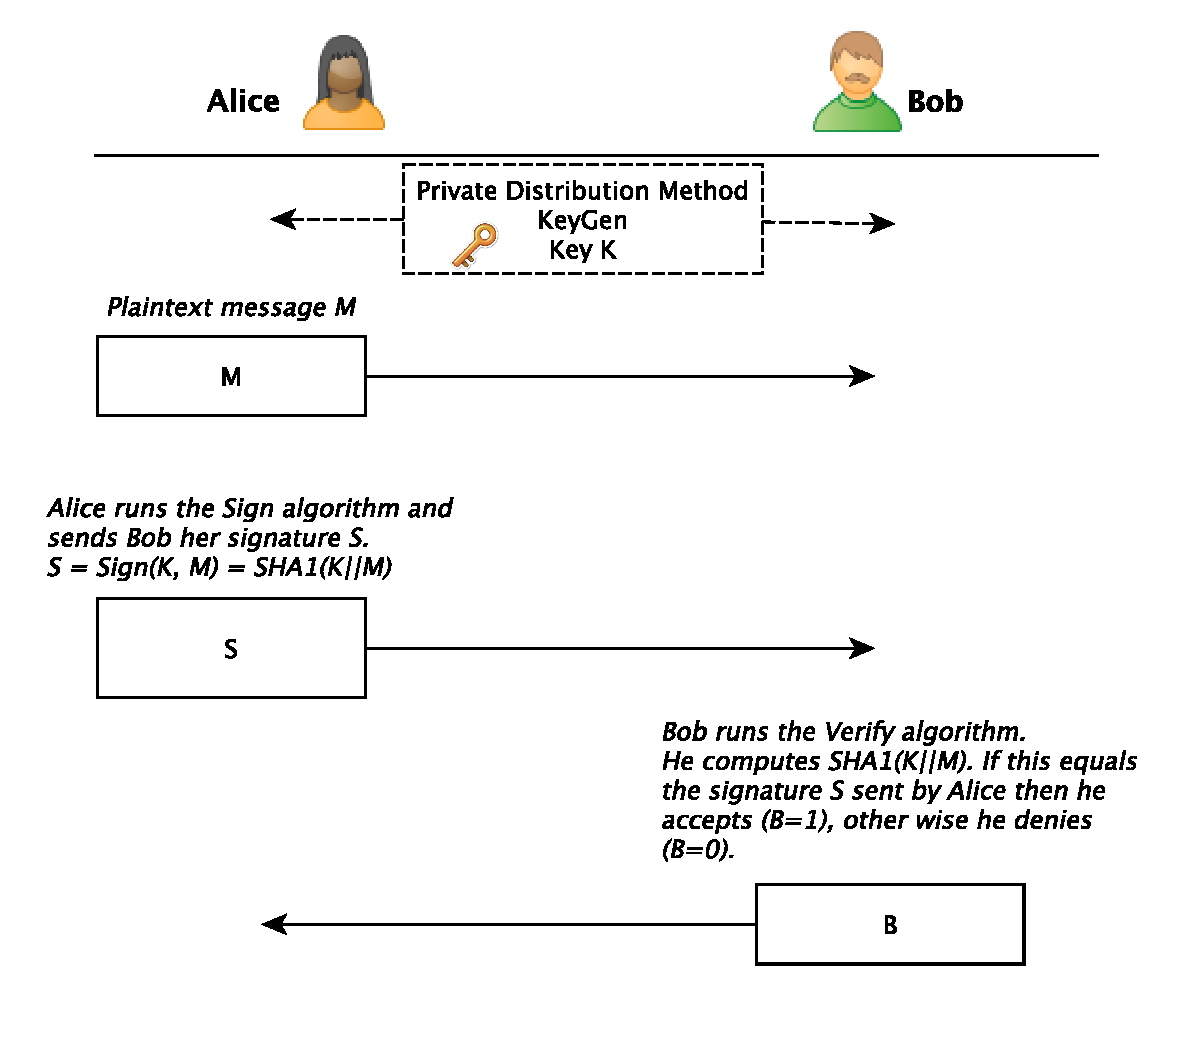
\includegraphics[scale=.4]{IMG/LEA1}
\end{figure}
\end{frame}

\begin{frame}
\frametitle{SHA-1: Length Extension Attack}

Eve could attack as follows.
\begin{figure}
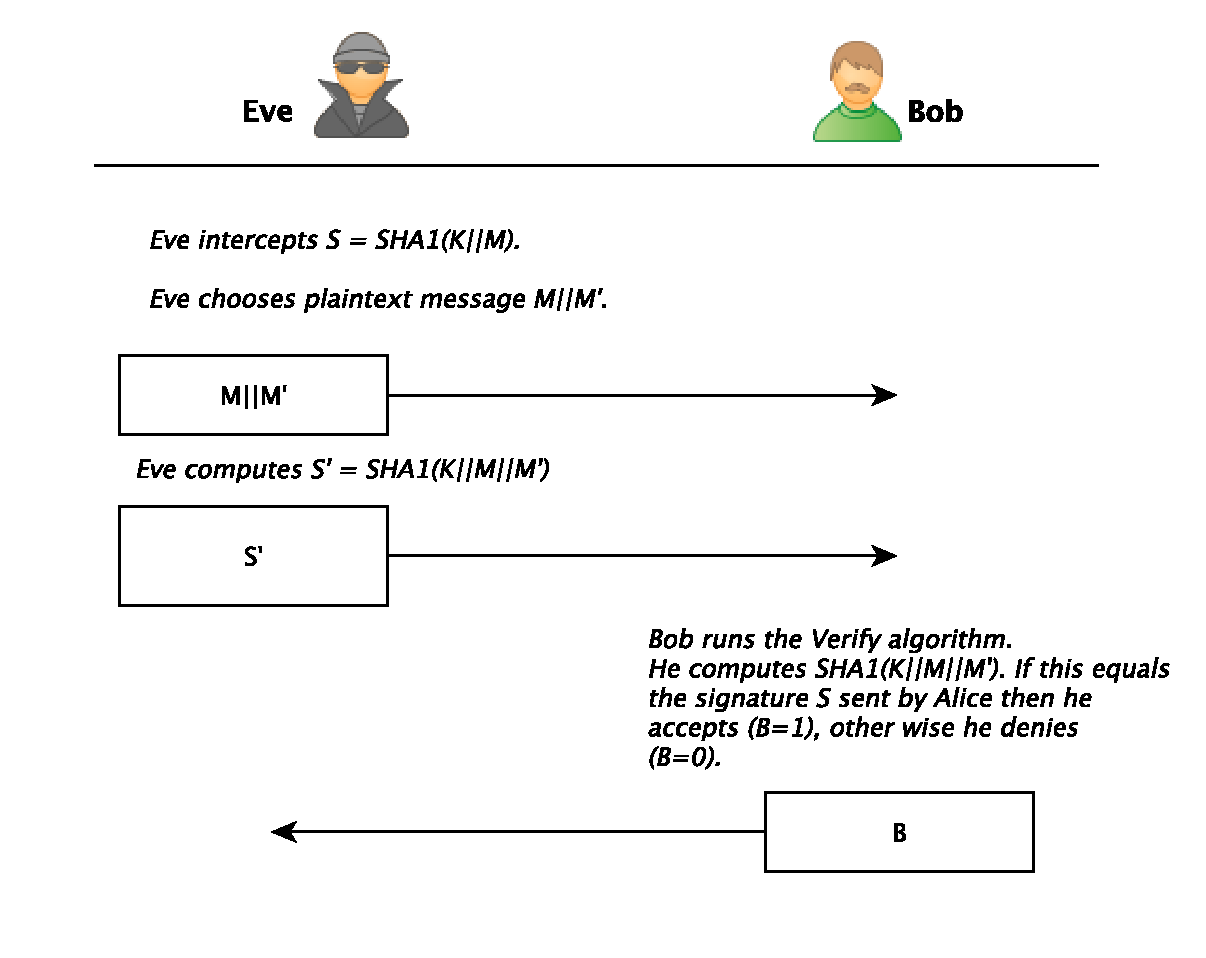
\includegraphics[scale=.45]{IMG/LEA2}
\end{figure}
\end{frame}


\begin{frame}
\frametitle{How to protect against this attack}

Avoid the Merkle-Damgard construction! Instead use something like HMAC (with nested hashing). \newline

Alternatively append a message number or a timestamp to the beginning of your message so that extending that message is pointless.
\end{frame}

\begin{frame}
\frametitle{References}

\begin{itemize}
\item \emph{Applied Cryptography} By Schneier, Chapter 18
\item \emph{Cryptography Engineering} by Schneier, Ferguson, Kohno, Chapter 6
\item \url{https://lord.io/blog/2014/length-extension-attacks/}
\end{itemize}
\end{frame}
\end{document}


